% Tex Resume 
% John R. Clayton 2017-04-26

% call to custom class file based on {article}
\documentclass[letterpaper]{twentysecond-charactersheet}

%%% Personal Information %%%

% Name
\cvname{John Clayton}

% Title
\cvjobtitle{Research Scientist}

% Date
\cvdate{April, 2017}
%\cvdate{\today}

% Set Timeline Range
\tlmaxdates{1996}{2015}

% Personal Photo
\profilepic{img/profile.png}

% About Me
\aboutme{}

% LinkedIn URL
%\cvlinkedin{https://linkedin.com/in/johnrandyclayton}
%\linkedinusername{johnrandyclayton}
\cvlinkedin{anon}
\linkedinusername{johnrandyclayton}



% GitHub URL
%\cvgithub{https://github.com/jrclayton/}
%\githubusername{jrclayton}
\cvgithub{https://www.google.com}
\githubusername{anon}


% Quora URL
%\cvquora{https://www.quora.com/profile/John-Clayton-6}
%\quorausername{John-Clayton-6}
\cvquora{https://www.google.com}
\quorausername{anon}

% Phone number
\cvnumberphone{+1 (555) 555--1212}
\cvnumbersimple{15555551212}

% Skype
%\skype{jrclayton}
\skype{anon}

% Email
%\cvmail{jrclayton@yahoo.com}
\cvmail{anon@gmail.com}

% QR Code Text
\qrtext{https://raw.githubusercontent.com/jrclayton/JRC-charactersheet/master/JRC-resume.pdf}

% Logo Width
\logowidth{32pt}

% Command for printing skill bubble diagram
\newcommand\skills{%
	\smartdiagram[bubble diagram]{%
		{Molecular} \\ {Biology},
		{~~~Virology~~~},
		{Parasitology},
		{~Entomology~},
		{~~Genomics~~},
		{Biostatistics},
		{Bioinformatics}
	}
}

% Programming skills (6.55)
\programming{{Python/3},{\small{\LaTeX}/4},{Bash/4},{R/5.24}}

% Language skills (6.55)
\languages{{German/1.75},{Spanish/3.25},{French/4.25},{English/6.55}}

%%% Begin Typesetting %%%
\begin{document}

% Print the sidebar with info from the preamble above
\makesidebar
% Sets up the header as a tikz image at the top of the page
\header{John}{Clayton}{Research Scientist}

% A Fun Quote
\myquote{The endless wonder of science is that the more we know, the more we know there is to know}{-- Stephen Budianski}

\vspace{46pt}

% Experience
\section{Experience}

% CV ENTRIES with modified MODERNTIMELINE macro

\tlcventry{2015}{2011}%
	{Post-doctoral Scholar}{Strasbourg, France}%
	{
\includegraphics[width=\logowidth]{img/INSERM.png}}%
	{\href{http://www-ibmc.u-strasbg.fr/}{\emph{Institut national de la sant\'{e} et de la recherche m\'{e}dicale} \acr{(INSERM)}\\Universit\'{e} de Strasbourg}}%
	{\begin{itemize}
			{\item[\color{gold}\faStar] successfully developed molecular reagents for allele-specific \acr{RNAi} in \emph{Anopheles gambiae}}
		\end{itemize}
		\begin{itemize}
			{\item[\color{gold}\faStar] used small-\acr{RNA}-seq to identify \acr{piRNA}-like small \acr{RNAs} derived from a transgene locus}
		\end{itemize}
	}

\tlcventry{2010}{2003}%
	{Pre-doctoral Researcher}{Baltimore, MD USA}%
	{
\includegraphics[width=\logowidth]{img/JHSPH.png}}%
	{\href{http://www.jhsph.edu/departments/w-harry-feinstone-department-of-molecular-microbiology-and-immunology/}{Johns Hopkins Bloomberg School of Public Health\\Department of Molecular Microbiology \& Immunology}}%
	{\begin{itemize}
			{\item[\color{gold}\faStar] characterized an acquired, sequence-specific anti-viral resistance observed in \emph{Aedes aegypti} during virus infection}
		\end{itemize}
		\begin{itemize}
			{\item evaluated recombinant Alphaviruses expressing pro-apoptotic genes as a potential biocontrol agents}
		\end{itemize}
	}

\tlcventry{2003}{2002}%
	{Post-baccalaureate Researcher}{Heidelberg, Germany}%
	{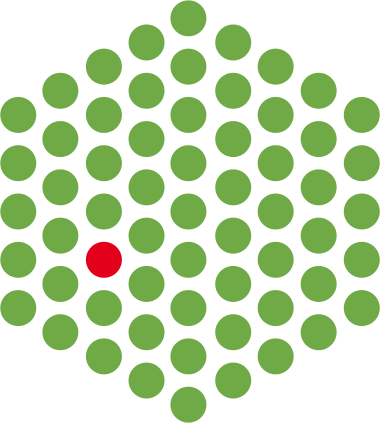
\includegraphics[width=\logowidth]{img/EMBL.png}}%
	{\href{http://www.embl.de/}{European Molecular Biology Laboratory}}%
	{\begin{itemize}
			{\item[\color{gold}\faStar] identified a role for a Rel-family transcription factor during \emph{Plasmodium} infection of mosquitoes}
		\end{itemize}
		\begin{itemize}
			{\item developed strains of transgenic \emph{Anopheles gambiae} expressing \acr{eGFP} in dying epithelial cells invaded by the malaria parasite}
		\end{itemize}
	}

\tlcventry{2002}{2000}
	{Emerging Infectious Diseases Fellow}{Atlanta, GA USA}
	{
\includegraphics[width=\logowidth]{img/CDC.png}}%
	{\href{http://www.cdc.gov/}{Centers for Disease Control and Prevention}}
	{\begin{itemize}
			{\item[\color{gold-metallic}\faTrophy] developed the genetic transformation method for \emph{Anopheles gambiae}}
		\end{itemize}
		\begin{itemize}
			{\item assisted in \acr{CDC} response during the 2001 Anthrax bioterror crisis}
		\end{itemize}
	}

% Education
\section{Education}

	\tlcventry{2010}{2003}%
		{Doctorate}{Baltimore, MD USA}%
		{
\includegraphics[width=\logowidth]{img/JHU.png}}%
		{\href{http://www.jhsph.edu/departments/w-harry-feinstone-department-of-molecular-microbiology-and-immunology/}{Johns Hopkins Bloomberg School of Public Health\\Department of Molecular Microbiology \& Immunology}}%
        {\vspace{-24pt}\begin{itemize}{\item Dissertation: \emph{Transduction of Virulence Factors by Alphaviruses in Vertebrate \& Invertebrate Models of Infection}}\end{itemize}}%

	\tlcventry{2005}{2003}%
        {Certificate in Vaccine Science \& Policy}{Baltimore, MD USA}{}%
        {\href{http://www.jhsph.edu/departments/international-health/}{Johns Hopkins Bloomberg School of Public Health\\Department of International Health}}{}%

	\tlcventry{2000}{1996}%
		{Bachelor of Arts}{Berkeley, CA USA}%
		{
\includegraphics[width=\logowidth]{img/cal.png}}%
		{\href{http://mcb.berkeley.edu/}{University of California at Berkeley\\Deptartment of Molecular \& Cell Biology}}%
		{\vspace{-24pt}{\begin{itemize}{\item Emphasis: \emph{Genetics \& Development}}\end{itemize}}}%

% QR Code in bottom right corner
\vspace{-24pt}
\qrgen{\qrtext}

\end{document}